\chapter[De l'individu à la population: quand la densité dépendense casse la
règle taille~--~température][Densité dépendance et température]{De l'individu à la population: quand la densité dépendance casse la
règle taille~--~température}
\label{Ann:fip}

\vspace{2cm}

\texttt{
Mallard, François, Vincent Le Bourlot, Christie Lecoeur, and Thomas Tully, ``From
individuals to populations:
density dependence effects break the temperature-size rule''\\
under review at Journal of Animal Ecology
}

\section*{Abstract}
\addcontentsline{toc}{section}{Summary}

\lettrine[lines=3]{D}{ensity-dependence} complicates the task of predicting the
effect of climate change on populations. Life history traits are known to be
plastic in response to temperature change: adult size of most ectotherms follows
the so-called temperature-size rule. Life history traits are also known to be
density dependent. In turn, density-dependence may be modulated by temperature.

Our aim is to disentangle the effects of temperature, density dependence and
their interaction on body length. Do to this we compare the thermal reaction
norms measured on isolated individuals, and on long time series of entire
populations.

Using the Collembola Folsomia candida, we describe the reaction norms of
maturation length, growth rate and asymptotic size over a large temperature
range (11 to 26$\degres$C) and examine the structure and dynamics of populations
reared under the same temperatures for three years. We use these reaction norms to
predict variation of adult size and growth rates measured in the populations.

We found that the body length of isolated individuals follow the
temperature-size rule. The population dynamics and population size structure
also depend on temperature, but individual-level reaction norms are overruled by
density dependent effects. At high temperature, the adults reach a higher body
size while the population density decreases, which may result from a more
intense interference competition between individuals.

This underlines the need to untangle the complex interactions between
environment and demography to help predicting how climate change influences
population dynamics.


\section{Introduction}

Long-term studies of natural populations have shown that climate change can lead
to shifts in life history trait with direct consequences on the population
dynamics \autocites{parmesan2006a,ozgul2009a,ozgul2010coupled}.
In the yellow-bellied marmot for instance, the recent increase of the active season mean duration allow the
individuals to reach larger body masses before winter. This lead to an increased
mean survival during hibernation and ultimately induce the population growth
\autocites{ozgul2010coupled}.

These shifts can originate from either ecological or evolutionary processes, or
the interaction of both
\autocites{ozgul2009a,pelletier2007evolutionary,kokko2007a,saccheri2006natural}.
The comprehension of the mechanisms that may allow species and community to cope
with climate change is a major issue of modern conservation biology
\autocites{lavergne2010a}. Both empirical and laboratory studies of
natural populations \autocites{edeline2013a,atkinson1996a}
have shown that temperature is a key abiotic factor influencing life history
traits \autocites{gillooly2001a}.

Warming can directly affect physiological rates such as consumption, digestion,
metabolic (both anabolic and catabolic) or respiration rates. These effects may
have demographic consequences such as increasing growth rates, earlier
maturation, and an overall acceleration of life cycles
\autocites{gillooly2002a,le-galliard2012a}. Associated with these physiological
changes, temperature is also known to induce phenotypic plasticity such as
modifications in resource allocation towards growth, reproduction or increased
survival
\autocites{liefting2010temperature,hallsson2012selection,gutteling2007mapping}.
One of the best-known life history pattern induced by temperature is the
temperature-size rule, which states that final adult body size is higher in cold
than in warm conditions.
This rule applies to a large number of endotherms and ectotherms
\autocites{atkinson1994a,atkinson1996a,angilletta2009a,walters2006temperature,daufresne2009global}.

Temperature change can also alter behavioural traits such as activity
\autocites{atacho2013a,seebacher2005review}, dispersal
\autocites{bonte2008thermal} or habitat choice
\autocites{vanbeest2012temperature}. Plastic changes induced by temperature
variations in ladybirds are a good illustration of the complex interactions of
the effects of temperature on physiology, behaviour, and melanism
\autocites{michie2010melanic}.

A classical approach to studying the influence of temperature on phenotypes is
by measuring reaction norms \autocites{woltereck1909a}, usually on isolated
individuals \autocites{driessen2007a,ellers2011b} or small cohorts
\autocites{liefting2009a,karan1998a} reared in the laboratory over a range of
temperatures. Although these laboratory experiments can tell us a lot about how
environmental conditions alter individual phenotypes, their applicability to the
way a population or a community responds to environmental change may be limited.
Indeed, temperature affects not only the physiology of each individual but also
the state of the population itself (in terms of abundance and structure). This
in turn affects the traits of individuals through density dependent processes.
Competition experiments have shown that temperature can alter population
dynamics or species diversity through modifications of competitive abilities
\autocites{park1954a,tilman1981competition}. In natural populations the direct
temperature effects on individual traits and the indirect effects through
density dependence are necessarily confounded. Different mechanisms have been
proposed to explain the temperature-dependence of these traits in natural
populations \autocites{sheridan2011a}.
Indeed, disentangling these two types of effects in natural population is a
difficult task.  For example, indirect effects of temperature such as prey size
variation can explain either negative \autocites{husby2011testing} or positive
\autocites{yom2008recent} influence on body length as a
consequence of warming.

We ask here whether thermal reaction norms measured on isolated individuals over
a large range of temperatures range can be used to predict population dynamics
and population structure over the same range of temperatures. We aim at
understanding how the direct effects of temperature on the life history of
individuals are modulated by demographic feedback, i.e., the density-dependent
processes due to interactions between individuals and their environment. To do
so we used the springtail Folsomia candida to measure the effect of temperature
at both the individual and the population levels. This soil arthropod is easy to
keep under laboratory conditions and is commonly used as a model organism in
evolutionary ecology and ecotoxicology
\autocites{fountain2005a,tully2005a,tully2008a,tully2011a}.

Our populations were bred with a constant amount of food, provisioned once a
week. We let the populations settle before measuring cohort growth rates and
adult body lengths. As stated in recent studies
\autocites{sheridan2011a,reuman2014metabolic}, if nutrient inputs remain
constant over a temperature gradient, and if the metabolic rates increase with
temperature, we can expect a demographic compensation either by a diminution of
the population size or by a reduction of the adult body lengths. By comparing
the demographics traits in our two contrasted demographic environments one can
assess the importance of competition in thermal body length adjustement.

The effect of temperature on competitive abilities has mainly been tested via
inter-specific experiments \autocites{park1954a,tilman1981competition} and
models \autocites{vasseur2005a,gilman2010framework}.
\textcites{ohlberger2012a} predict that an increased temperature is likely to
increase the size-asymmetry between individuals in freshwater fish populations
and therefore to favour smaller individuals in hotter environments.
\textcites{reuman2014metabolic} found a similar result in a recent model that
focused on phytoplankton dynamics. Thus, we expect in our experiment that
exploitative competition will induce an additional decrease of body length in
the populations compared to what may be observed on isolated individuals that
follow the temperature-size rule.

Other types of competition are known to affect body length depending on
temperature, such as nutrient storage abilities
\autocites{litchman2009contrasting} or direct interactions between individuals
\autocites{park1962a,schoener1983a,anholt1990a,smallegange2006a,nakayama2010a,mccormick2012a}.
In our experimental setting, competition can become fierce in populations:
juveniles and adults have the same ecology and share the same food resources.
Therefore it is likely that interference competition mediates the access to the
resource. Interference between individuals reduces the individuals’ feeding
rates because of the time spent interacting with others to the detriment of
feeding \autocites{smallegange2006a} and because of the extra energetic
cost associated with these agonist interactions \autocites{briffa2007a}.
In case of a significant difference in size and strength between the interacting individuals, the
dominants deny the smaller individuals access to resources with a minimal
effort. Therefore the cost of interference for the dominating individual is
negligible whereas it is maximal for the smaller ones.
This counteracts the effect of exploitative competition with consequences on the
size structure of the population (Le Bourlot et al. submitted). Yet, it is not
clear how temperature affects interference competition. An increase of
temperature could weaken interference competition by reducing population size.
But it could also increase interference competition by an increase of individual
activity.


\section{Material and methods}

\subsection{Model organism}

The Collembola Folsomia candida is a small ($\sim 2$mm long) blind ametabolous
hexapod, broadly distributed throughout the world. It is found in habitats such
as decaying litter, rotting wood or in caves \autocites{fountain2005a}. It
is easy to maintain in the laboratory, and can be bred in isolation or in populations in
very simplified microcosms with a fine control of the main parameters
(temperature, food, density, humidity). Every life cycle stage is visible (eggs,
nymphs, adults). Measurements and environmental manipulations can be done on
both nymphs and adults since they share the same environment, eat the same food
and have the same ecology {Fountain 2005}. Individuals grow by moulting about
twice a week at $21\degres$C during their whole lifetime. As ectotherms, the
developmental rate and rythm of moulting and egg laying increase with
temperature \autocites{cutkomp1986chronobiologic}. Each individual eat between every
moult and lay a clutch every two moults \autocites{palevody1974a}. Thus
at $21\degres$C, an individuals needs to eat twice a week.

This species is known to demonstrate highly flexible phenotypic adjustments when
experiencing a sudden change in density or resource abundance \autocites{tully2008a}.
As a parthenogenetic species, multiple individuals sharing the same genotype can
easily be bred in different environmental conditions. We worked with two
distinct genetic clonal lineages (labelled respectively TO and HA) with
contrasted ecological history and bio-demographic strategies
\autocites{tully2006a,tully2008a}.

\subsection{Rearing conditions}

Both isolated individuals and populations were kept in standard rearing boxes
made of polyethylene vials (diameter 52 mm, height 65 mm) filled with a 30 mm
layer of plaster of Paris mixed with 600 mL of Pébéo graphic\circledR Chinese
ink to increase visual detectability of light individuals against the dark
background \autocites{tully2008a}. In isolation, resource was provided ad
libitum. In populations, food was provided once a week in the form of small
pellets of a mixture of dried yeast and agar in standardized concentration and
volume (5000 mL water+80 mg agar+800 mg dried yeast, to produce pellets of 15
$\mu$L). Both isolated individuals and populations were kept in incubators (Velp
FOC 225E, temperature controlled $\pm$0.5$\degres$C), at constant humidity ($\sim
100\%$) and in darkness.

\subsection{Thermal reaction norms of isolated individuals}

Newborns were isolated immediately after hatching and fed ad libitum during
their whole life. We randomly placed individuals of each clone at each
temperature within our range (11, 16, 21, 26 and 29$\degres$C). The body length
of the individuals was measured three times a week during ten weeks, starting the first
day of the experiment, and then once a week (Figure \ref{fig:AnFIP1} and
Supplementary Materials Figure \ref{Fig5-S1}).
For each body length measurement, two to three pictures were taken using a digital camera (Nikon D300) fixed on a
dissecting scope. Body length was measured on each picture using the ImageJ
software \autocites{abramoff2004a} (\url{http://rsbweb.nih.gov/ij/}). The
containers were regularly inspected for eggs to assess age at maturation. Logistic growth curves
were fitted to each individual growth trajectory. Average maximal
growth rates and asymptotic sizes were estimated using non-linear least squares
models fitted separately for each individual growth trajectory using the methods
described by Pinheiro and Bates \autocites{pinheiro2000a}. Linear models were
used to test for fixed effects (clonal identity and temperature being used as categorical
variables) on these two parameters using anova F-tests.

\begin{figure}[!ht]
\begin{center}

\includegraphics[width=\textwidth]{1_CorpsDeThese/Resumes/Fig/FIP01}
\caption[\lofimage{1_CorpsDeThese/Resumes/Fig/FIP01}Growth
trajectories]{Individual growth trajectories for clone HA (a-d)
and TO (e-h) at $11$ (a and e), 16 (b and f), 21 (c and g) et $26\degres$C (d and
h).}
\label{fig:AnFIP1}
\end{center}
\end{figure}

% 
% \begin{table}[!ht]
% \centering
% \caption{
% Number of isolated individuals followed since birth and populations followed
% during more than one year of the two clones and for the four temperatures. The
% number of individuals whose asymptotic length has been observed is in
% brackets.}\label{tab5-1}
% \begin{tabular}{ccccc}
% \hline
% \multirow{2}{*}{temperature} 
% 	& \multicolumn{2}{c}{Number of isolated individuals}
% 	& \multicolumn{2}{c}{Number of populations}\\
% %case vide
% 	& HA
% 	& TO
% 	& HA
% 	& TO\\
% \hline
% 11$\degres$C 
% 	& 4 (5)	
% 	& 5 (4)	
% 	& 4	
% 	& 4\\
% 16$\degres$C
% 	& 6 (5)	
% 	& 9 (8)	
% 	& 4	
% 	& 4\\
% 21$\degres$C
% 	& 7 (4)	
% 	& 6 (2)	
% 	& 12 
% 	& 12 \\
% 26$\degres$C
% 	& 6 (5)	
% 	& 9 (7)	
% 	& 4	
% 	& 4 \\
% \hline
% \end{tabular}
% \end{table}

\subsection{Population dynamics and cohort growth rates measurements}

Populations were started with five adults and maintained at the same
temperatures as the isolated individuals (11, 16, 21 and 26$\degres$C). To avoid
any transient effect, we analysed the dynamics of these populations after being
maintained during at least one year at these temperatures. Four populations were
started for each clone at each temperature, and an extra eight populations per
clone were added at 21$\degres$C.

The population size structure was measured weekly during more than a year using
a dedicated plugin \autocites{mallard2013a,mallard2012a} of the ImageJ software
\autocites{abramoff2004a} (\url{http://rsbweb.nih.gov/ij/}). Each
measurement gave us the number of individuals and for each individual counted, its length and its surface
(which we refer to as its biosurface). We extracted the life history traits
(adult body length and juvenile growth rate) in populations using the graphical
representation for structured time series (Figure \ref{fig:AnFIP2}) provided by
the R package STdiag (\url{http://stdiag.r-forge.r-project.org/}).

\subsection{Thermal reaction norms of demographic traits}

We measured juvenile growth and adult body length on the population dynamics
structured-time diagrams using cohorts growing within the group of adults
(Figure \ref{fig:AnFIP2}). The growth rate of each cohort was measured by taking the slope
of the mean body length in the cohort against time. Finally, the asymptotic
adult body length of each cohort was taken as the average length of the adults
once the growing cohort fully merged with the pre-existing adults, or when the
average length of the growing cohort stabilizes (Figure \ref{fig:AnFIP2}). We
extracted the number of individuals and the size of each individual during the
periods of measurements. This count was used to measure the density of adults at
the time of each measurement. Individuals are considered as adults if their
length is greater than 0.8mm.

\newpage

\begin{figure}[H]
\begin{center}
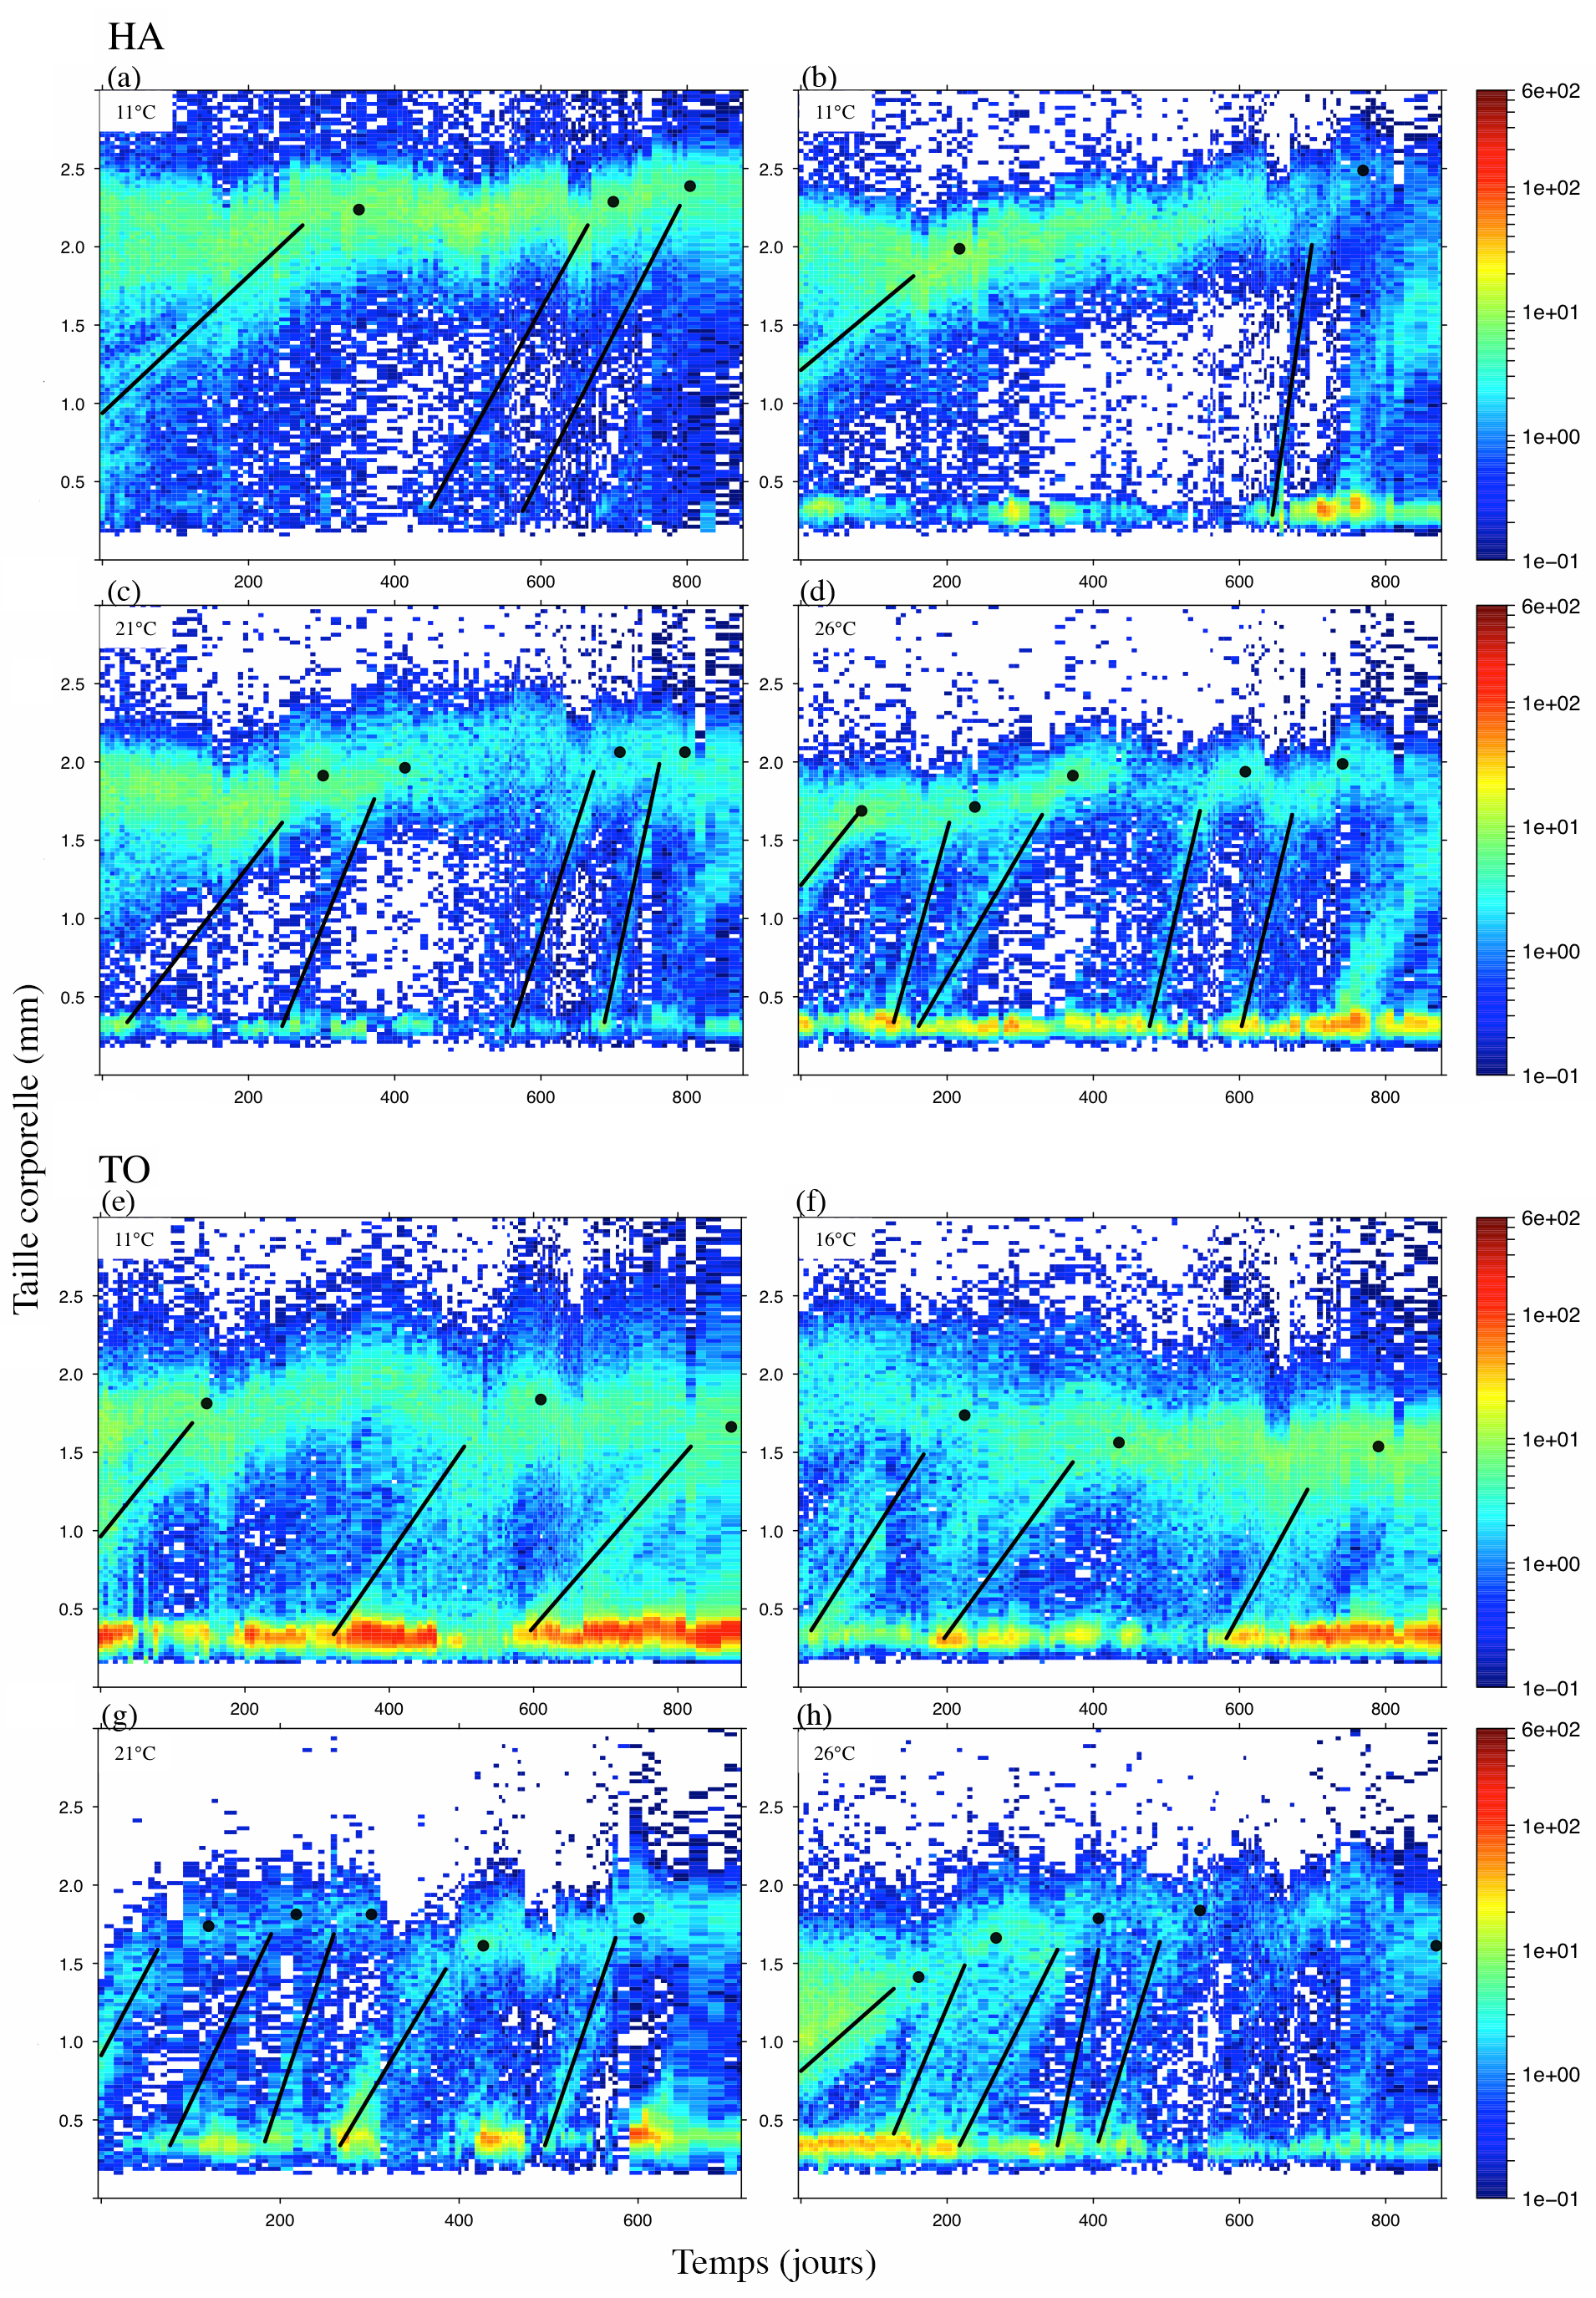
\includegraphics[width=\textwidth]{1_CorpsDeThese/Resumes/Fig/FIP02}
\caption[\lofimage{1_CorpsDeThese/Resumes/Fig/FIP02}Examples of
structure time diagrams]{Examples of
structure time diagrams for clones
HA (a-d) and TO (e-h) at $11$ (a and e), 16 (b and f), 21 (c and g) and
$26\degres$C (d and h). Points mark measures of adult body length, lines mark
measures of cohort growth rates.}
\label{fig:AnFIP2}
\end{center}
\end{figure}

\subsection{Measuring the thermal reaction norms for growth rate and adult size
in populations}

In populations the changes in growth rates and asymptotic adult body lengths are
attributed to direct effects of temperature, direct effects of population
density, and potential interactions between temperature and density. To
specifically focus on the effects of density (possibly in interaction with
temperature) while controlling for the direct effects of temperature (thermal
reaction norms on isolated individuals), we used two indexes that compare the
traits measured in populations with the measurements made on isolated
individuals, rather than directly analysing the growth rates and adult length in
populations.

For growth rates we used a linear model explaining the ratio between the
observed growth rates in the populations and the average maximal growth rate of
isolated individuals at the same temperature. We call this ratio the ``relative
growth rate in population''. The logarithm of adult density (number of adults in
the container at that time), the temperature (used as a continuous variable
here), the clonal lineage and their interactions were used as explanatory
variables.

Similarly, in order to determine the roles of temperature and density dependent
processes in the regulation of adult body length in populations, we compared the
lengths of adults in populations to that of isolated individuals. More
precisely, we created an index called the ``Growth effort beyond maturation''
(GEBM) to look at the individual’s investment in body length after reaching
maturity when in populations. The GEBM depends on temperature and represents the
proportion of the length that adults grow to in addition to the maturation
length. The maturation and the asymptotic body lengths measured on isolated
individuals are used as references for scaling the average adult body lengths
observed in the populations.


\begin{equation}
GEBM(T)=\frac{\text{Adult body length}_{\text{populations}}(T) -
\text{Length at maturity}_{\text{individuals}}(T)}{\text{Adult body
length}_{\text{individuals}}(T) -
\text{Length at maturity}_{\text{individuals}}(T)}
\end{equation}
 
For a given temperature, the maturation and asymptotic body length being known
in isolation, the GEBM shows how far individuals continue growing after maturity
with respect to measurements on isolated individuals. GEBM=0 means that the
adults ceased growing after reaching maturity. GEBM=$50\%$ indicates that the
individuals grew half way to the asymptotic length reached by isolated
individuals. Values below 0 or exceeding $100\%$ indicate that individuals in
populations are respectively smaller than the length at maturity of isolated
individuals or reach a greater length than when kept isolated.

To calculate growth effort beyond maturation we pooled the measurements of
length at maturity and adult length of isolated individuals made on the two
clonal lineages, as we found no statistical differences between them. Then we
analysed GEBM using linear models with adult density, temperature (as
categorical variable here because of its non linear effect, see below) and the
clone identity as explanatory variables with all possible interactions. As for
the analysis of growth rate, we used linear models (lm from the stats package
from R software \autocites{pinheiro2000a}) with ``population'' included as a
random factor since several measurements could have been taken from the same population. We
simplified the models using a backward elimination procedure (drop function in
R). Statistical significance of the fixed effects and their interactions were
assessed with anova F-tests. All analyses were implemented using R 3.0.2
software (http://cran.r-project.org \autocites{ihaka1996a}).


\section{Results}

\subsection{Thermal reaction norms}

\subsubsection{Growth rates}

The growth rate of isolated individuals increased almost linearly with
temperature (Figure \ref{Fig5-3}). At 11$\degres$C, both lineages had similar
growth rates (F$_{1,36}=2.6$, p$=0.12$). But the slope of the growth rate
increase with temperature was higher for TO than for HA (HA: $2.4e-03
mm.\degres$C$^{-1} \pm SE = 3.4e-04$, mean difference between lineages is
$1.4e-03 \pm SE = 3.4e-04$, $F_{1,37} = 18$, $p = 0.0002$). As a consequence,
the mean growth rate at $26\degres$C was $25\%$ lower for HA individuals than
for TO ones ($F_{1,10} = 12$, $p = 0.006$). The cohorts in populations grew much
slower than the isolated individuals did at all temperatures Figure \ref{Fig5-3}a,b). On
average, HA juveniles grew faster than TO ones (the difference being $-2.3e-03
mm.day^{-1} \pm SE = 1.1e-03$, $F_{1,148}=4$, $p=0.04$). But warming had the
same linear positive effect on both lineages: an increase of $1\degres$C causes
the growth rate to rise by $6.6e-04 mm/day$ ($F_{1,148}=26$, $p<0.0001$).

\begin{figure}[!ht] % Figure 3 
\centering
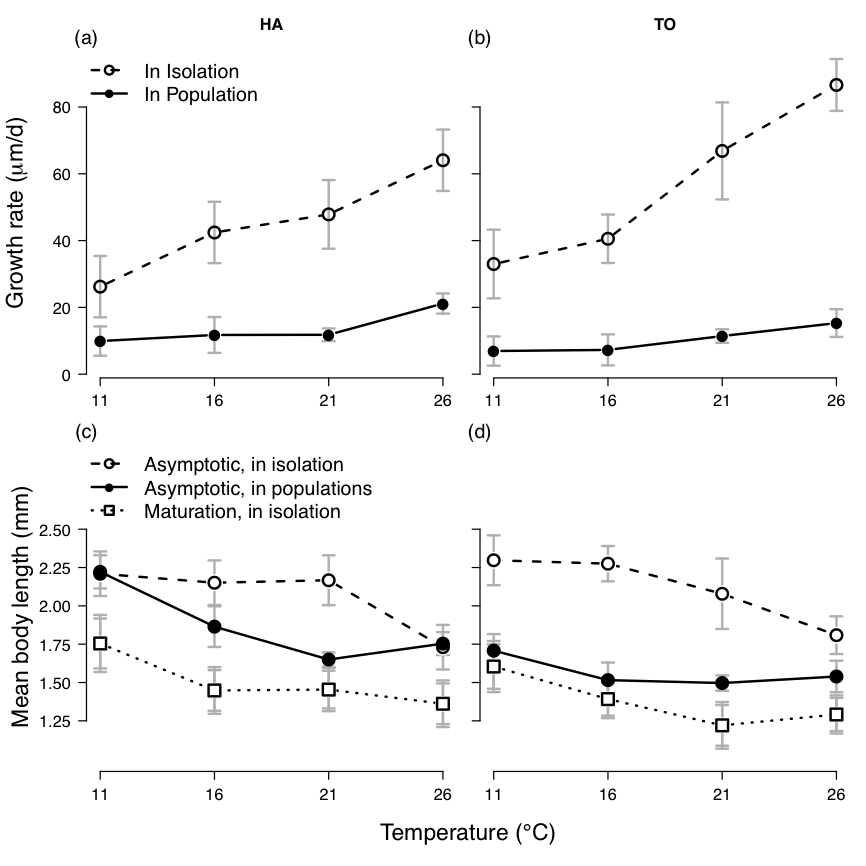
\includegraphics[width=0.80\textwidth]{1_CorpsDeThese/Resumes/Fig/FIP03} 
\caption[\lofimage{1_CorpsDeThese/Resumes/Fig/FIP03}Thermal reaction norms of the growth
rates]{ Thermal reaction norms of the growth rates (a, b, mean and 95\% confidence intervals) of the clones HA (a) and TO (b) measured on isolated individuals (dashed lines)
and on cohorts within populations (strait lines). Thermal reaction norms for
mean body length (c, d): mean body length at maturity (dotted lines) and
asymptotic length of isolated individuals (dashed lines) compared with mean
adult body length in populations (strait lines).}
\label{Fig5-3}
\end{figure}

\subsubsection{Maturation and asymptotic size}

Isolated individuals of both strains followed almost identical thermal reaction
norms for maturation and asymptotic sizes (Figure \ref{Fig5-3}c,d). First,
asymptotic size decreased with temperature ($-0.033 mm/\degres$C $\pm SE =
3.9e-03$, $F_{1,38} = 73$, $p < 0.0001$) without any difference between the
clonal lineages: the mean slope ($F_{1,36} = 0.97$, $p = 0.33$) and the
intercept at $11\degres$C ($F_{1,37} = 2.1$, $p = 0.16$) were identical for TO
and HA. Second, size at maturity at $11\degres$C was higher in the HA
individuals than in the TO ones ($0.12 mm \pm SE = 0.05$, $F_{1,49} = 5.5$, $p =
0.024$).
It then decreased with an increase of temperature ($-0.020 mm/\degres$C $\pm
SE=0.005$, $F_{1,50} = 17$, $p = 0.0001$) similarly for the two clones
($F_{1,48} = 0.06$, $p = 0.82$).

In contrast to isolated individuals, the effect of temperature on the mean adult
length in the populations differed between the two clones ($F_{1,3}=35,
p<0.0001$).
In cold environments, the HA individuals reached a size that did not differ from
the mean asymptotic sizes of isolated individuals (at $11\degres$C: $F_{1,61} =
0.01$, $p = 0.91$). Then, when temperature increased up to $21\degres$C, the
mean adult length in the HA populations progressively decreased and became close
to the mean maturation size (mean decrease = $-0.055 mm/day/\degres$C, $F_{1,61}
= 106$, $p < 0001$).
Remarkably, the mean adult length in the populations finally increased when the
temperature rose from $21\degres$C to $26\degres$C ($0.021 mm/day/\degres$C $\pm
SE=0.009$, $F_{1,65} = 5$, $p = 0.025$).
TO cohorts in populations stopped growing shortly after reaching their expected
size at maturity in cold environments: both values did not differ at
$11\degres$C ($F_{1,15} = 1$, $p = 0.31$)  and $16\degres$C ($F_{1,22} = 3$, $p
= 0.10$).
The mean adult length in the TO populations remained constant between
$16\degres$C and $26\degres$C ($F_{1,57}=0.2$, $p=0.82$) and was seen to be
higher than the length at maturity in isolation ($F_{1,23}=19$, $p=0.0002$) and
lower than the asymptotic length of isolated individuals ($F_{1,23}=20$,
$p=0.0002$, Figure \ref{Fig5-3}d).


\subsection{Density dependence and temperature}

To further investigate the differences between the thermal reaction norms in
isolation and in populations, we have studied how the relative growth rates and
GEBM of both lineages respond to temperature and population density. We used the
adult density as a proxy of the population state since adult represents on
average $90\%$ of the total biosurface in our populations and since we know from
other experiments that adults outcompete juveniles in resource acquisition and
therefore play a central role in the density dependence effects (Le Bourlot et
al. under review).

\subsubsection{Density dependence and relative growth rates}

For each temperature, the relative growth rate of cohorts of juveniles decreased
exponentially with adult density (Figure \ref{fig:AnFIP4}, Table
\ref{tab:AnFIP1}).
HA juveniles grew on average faster than TO ones ($F_{1,153} = 17$, $p < .0001$)
but they suffered from a stronger negative effect of density ($F_{1,153} = 13$,
$p = 0.0004$). Therefore, the genetic difference progressively disapears with
increasing density. Finally, warming reduces the cohorts’ relative growth rates
($F_{2,153} = 52$, $p < .0001$). This effect is slightly lower for the TO
lineage ($F_{1,153} = 4$, $p = 0.048$) but this is certainly due to the lower
growth rate of the TO individuals at low density.

\begin{figure}[!ht]
\begin{center}

\includegraphics[width=\textwidth]{1_CorpsDeThese/Resumes/Fig/FIP04}
\caption[\lofimage{1_CorpsDeThese/Resumes/Fig/FIP04}Relative growth rates]{The relative growth rates ($\%$ growth rate in populations compared to
the growth rates measured on isolated individuals) and adult densities (number
of adults in a rearing box) measured in the populations raised under four
different ambient temperatures for the HA (dashed lines, open symbols) and TO
lineages (plain lines, filled symbols).}
\label{fig:AnFIP4}
\end{center}
\end{figure}

\begin{table}[!ht]
\centering
\caption{\label{tab:AnFIP1}Results of the linear model that analyse the cohort relative growth rates in the populations.}
\scriptsize
\begin{tabular}{rccccl}
\hline 
\multicolumn{6}{c}{$lm(\text{Growth rate} \sim (\log(\text{Adult density}) +
\text{Temperature}) * \text{Clone})$} \\
&&&&&\\
& Estimate & Std. Error & $t$ value & $\text{Pr}(>|t|)$ & \\
\hline

Intercept = Clone HA, Temperature 11 & $1.22e+00$ & $8.59e-02$ & $1.42e+01$
& $<2e-16$ & $***$\\

$\log(\text{Adult density})$ & $-1.48e-01$ & $1.34e-02$ & $-1.10e+01$ & $<
2e-16$ & $***$\\

$\text{Temperature}$ & $-1.57e-02$ & $1.82e-03$ & $-8.60e+00$ & $8.61e-15$ &
$***$\\

$\text{CloneTO}$ & $-4.90e-01$ & $1.18e-01$ & $-4.15e+00$ & $5.56e-05$ & $***$\\

$\log(\text{Adult density}):\text{CloneTO}$ & $6.79e-02$ & $1.86e-02$ &
$3.65e+00$ & $3.61e-04$ & $***$\\

$\text{Temperature}:\text{CloneTO}$ & $5.24e-03$ & $2.63e-03$ & $2.00e+00$ &
$4.79e-02$ & $*$\\

\hline 
\end{tabular} 
\end{table}

\subsubsection{Growth effort beyond maturation}

In most of the populations the observed body lengths were distributed bimodally
(see Figure \ref{fig:AnFIP2}). We were then able to discriminate the newborns from
the adult cohort and to estimate their density and mean body length from which we
calculate the Growth Effort Beyond Maturation (GEBM). In these populations we
found that the response of GEBM to adult density and temperature differed
quantitatively but not qualitatively between the two lineages (Figure
\ref{fig:AnFIP5}, Table \ref{tab:AnFIP2}).
On average the growth effort of HA is higher than that of TO individuals at each
temperature independently (Table \ref{tab:AnFIP2}). But this difference between
the two lineages decreases slightly with temperature increase ($F_{3,117}=3.2$,
$p=2.1$). For both lineages the growth effort decreased with increasing density
(Table \ref{tab:AnFIP2}):
when the adult density increased, the mean size reached by the cohorts was
closer to the size of isolated at maturity. The intensity of this density
dependence (slope of the decrease) did not differ between the two lineages
($F_{1,111}=2.4$, $p=2.1$) but increased in hotter environments (Table
\ref{tab:AnFIP2}).

\begin{table}[!ht]
\centering
\caption{\label{tab:AnFIP2}Results of the linear model that analyse the GEBM measured in the populations.}
\scriptsize
\begin{tabular}{rccccl}
\hline 
\multicolumn{6}{c}{$lm(GEBM \sim (\text{Adult density} + \text{Clone}) *
\text{Temperature})$} \\
&&&&&\\
& Estimate & Std. error & $t$ value & $\text{Pr}(>|t|)$ & \\
\hline

Intercept = Clone HA, Temperature11 & $2,01E+00$ & $1,93E-01$ & $1,04E+01$ & $< 2e-16$ & $*** $\\
Temperature16 & $-5,43E-01$ & $2,43E-01$ & $-2,23E+00$ & $2,77E-02$ & $* $\\
Temperature21 & $-9,25E-01$ & $1,98E-01$ & $-4,68E+00$ & $8,18E-06$ & $*** $\\
Temperature26 & $-7,06E-02$ & $2,10E-01$ & $-3,37E-01$ & $7,37E-01$ & $ $\\
Adult density & $-6,72E-03$ & $1,50E-03$ & $-4,48E+00$ & $1,84E-05$ & $*** $\\
CloneTO & $-7,62E-01$ & $7,88E-02$ & $-9,68E+00$ & $< 2e-16$ & $*** $\\
Adult density:Temperature16 & $2,35E-03$ & $1,77E-03$ & $1,33E+00$ & $1,87E-01$ & $ $\\
Adult density:Temperature21 & $3,76E-03$ & $1,53E-03$ & $2,46E+00$ & $1,56E-02$ & $* $\\
Adult density:Temperature26 & $-3,34E-03$ & $1,91E-03$ & $-1,75E+00$ & $8,36E-02$ & $. $\\
Temperature16:CloneTO & $1,58E-01$ & $1,15E-01$ & $1,37E+00$ & $1,73E-01$ & $
$\\
Temperature21:CloneTO & $2,48E-01$ & $8,80E-02$ & $2,82E+00$ & $5,71E-03$ & $**
$\\
Temperature26:CloneTO & $2,13E-01$ & $9,93E-02$ & $2,15E+00$ & $3,39E-02$ & $*
$\\

\hline 
\end{tabular} 
\end{table}

\begin{figure}[!ht]
\begin{center}
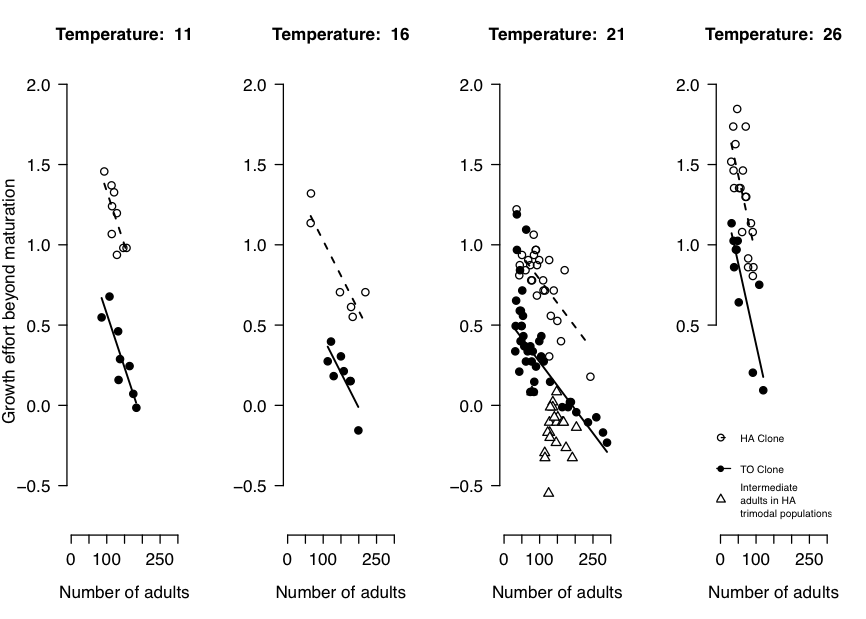
\includegraphics[width=\textwidth]{1_CorpsDeThese/Resumes/Fig/FIP05}
\caption[\lofimage{1_CorpsDeThese/Resumes/Fig/FIP05}The growth effort
beyond maturation]{The growth effort
beyond maturation, which is a measure of how much the individuals grow in the
populations compared to their body length when isolated, and population density
measured under four different ambient temperatures for the HA (dashed lines,
open symbols) and TO lineages (plain lines, filled symbols).}
\label{fig:AnFIP5}
\end{center}
\end{figure}

Some of the population dynamics of HA populations at 21$\degres$C led to a
trimodal size structure. In these populations, a first adult cohort reached a high length at
low density, followed by a second cohort that reached a lower mean body length
(see Supplementary Materials for examples). We found a
clear difference between those two sets of measurements: the GEBM of the first cohorts of larger
individuals followed the general model whereas the GEBM of the second cohorts
are not explained by the total number of adults in the population
($F_{1,19}=0.25$, $p=0.62$). Additional analyses performed on this data allowed
us to split the populations into three groups of individuals based on total length distribution
in the population: the juveniles, the intermediate adult class, and the large
adult class (see Supplementary Materials). We did not find any significant
correlation between the number of individuals in this intermediate adult class and their
GEBM ($F_{1,19} = 1.6$, $p = 0.2$). Instead, the number of
individuals in the large adult class correlates with both the number and the body length of the
adults in the intermediate class. We then calculated a final linear model to
explain the GEBM of all the HA cohorts at 21$\degres$C with the number of adults
in the larger cohort. We found no difference in the slope of the regression between the
GEBM and adult density of the two types of measurements ($slope = -0.0040 \pm SE
= 0.0005$, $F_{1,44} = 0.11$, $p = 0.74$), although there was a difference in
the intercept ($-1.04 \pm SE = 0.041$, $F1,45 = 656$, $p < 0.0001$). In other
words, the presence of a cohort of big adults in the population acts on the adults’ body
length exactly as if there were an additional 260 individuals of the same middle
size (i.e. the ratio between the difference in the intercept and the slope, see
Figure \ref{fig:AnFIP6}).

\begin{figure}[!ht]
\begin{center}

\includegraphics[width=0.75\textwidth]{1_CorpsDeThese/Resumes/Fig/FIP06}
\caption[\lofimage{1_CorpsDeThese/Resumes/Fig/FIP06}GEBM in populations of clone
HA at $21\degres$C]{GEBM measured in the HA populations for the cohorts of large
individuals ($\circ$) and of intermediate adults ($triangle$). The presence of
an extra cohort of large adults in the populations acts on these intermediate
ones as if there were an additional 260 individuals in the populations
($\ast$).}
\label{fig:AnFIP6}
\end{center}
\end{figure}

\subsubsection{Predicted thermal reaction norms}

For both lineages we also found that the GEBM varies with temperature. But
contrary to the growth rate, the effect of temperature was not linear. In order
to highlight how the relative growth rates and investment in growth (GEBM) vary
with temperature in our populations, while controlling for density within clonal
lineages, we plotted the predicted relative growth rate and the GEBM for a
density of 100 adults (the overall mean adult density observed in our
populations, Figure \ref{Fig5-5}a,b) using the models fitted to each lineage
independently (Table \ref{tab:AnFIP1} and Table \ref{tab:AnFIP1}). For both
lineages, the relative growth rate decreased linearly with increasing
temperature (Figure \ref{Fig5-5}a) but the GEBM reaction norms have a U-shaped
profile: GEBM decreased linearly as the temperature rose from 11$\degres$C to
21$\degres$C, but increased at 26$\degres$C (Figure \ref{Fig5-5}b). The body
length increase observed at 26$\degres$C compared to 21$\degres$C (Figure
\ref{Fig5-5}) is remarkable since in most of the populations maintained at
26$\degres$C, the mean adult body length was higher than the asymptotic length
of the isolated individuals at the same temperature (Figure \ref{fig:AnFIP6}c,d)
while in some HA populations maintained at 21$\degres$C some cohorts did not
even reach the length at maturity measured on isolated individuals (Figure
\ref{fig:AnFIP6}c, negative values).

\begin{figure}[!ht] % Figure 5
\centering
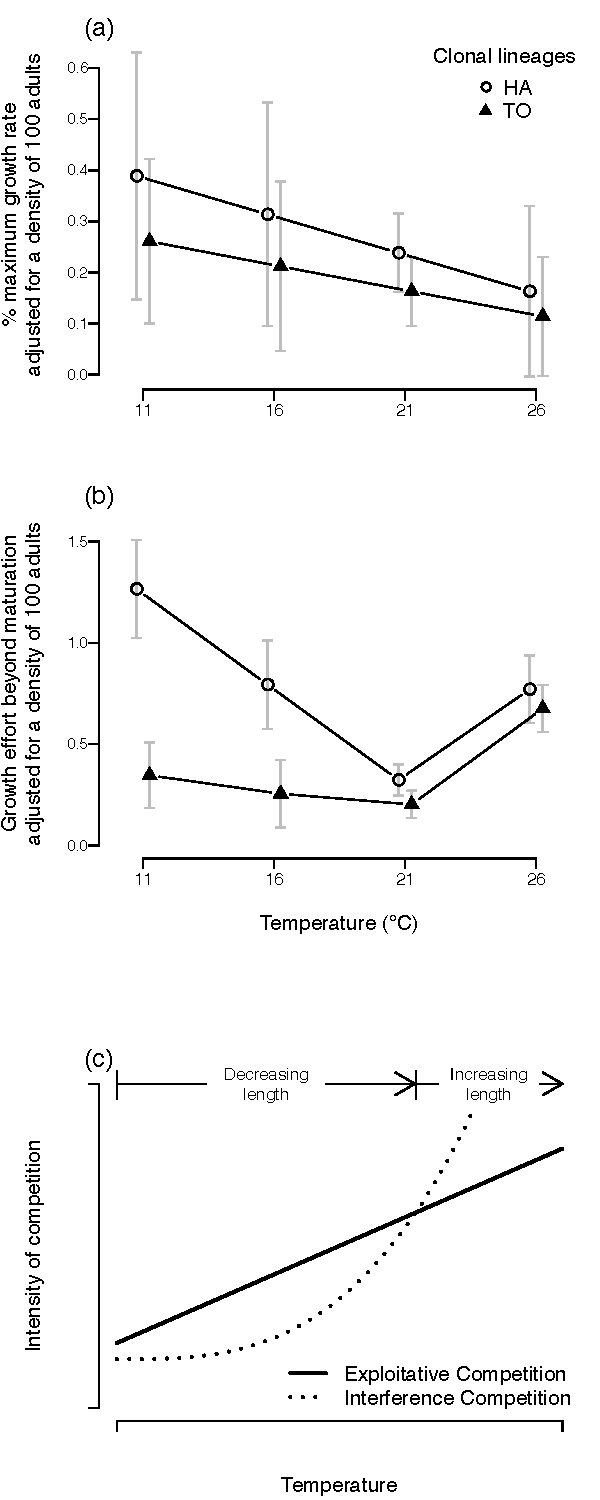
\includegraphics[height=0.8\textheight]{5_ChapExp3/fig/Fig5} 
\caption[\lofimage{5_ChapExp3/fig/Fig5}Thermal reaction norms of relative
growth rate and GEBM]{ The thermal reaction norms of relative growth rate (a)
and growth effort beyond maturation (b) for the two lineages. Predicted values from the fitted models
(mean ± 95\% confidence intervals) scaled for a density of 100 adults. (c)
Possible changes in the relative exploitative and interference competition in
the populations: as temperature increases, the intensity of interference
competition may prevail, thus favouring larger individuals.}
\label{Fig5-5}
\end{figure}

\section{Discussion}

\subsection{Thermal reaction norms of isolated individuals.}

The thermal reaction norms measured on isolated individuals revealed a positive
effect of temperature on the growth rate and a negative effect on adult body
length. From 11$\degres$C to 26$\degres$C, the average growth rate is multiplied
by three while the adult length decreases by about $20\%$. This proves that, as
with many other ectotherms \autocites{atkinson1994a,angilletta2009a}, the
Collembola \textit{F. candida} follows the temperature size rule: individuals
raised under cold ambient temperature grow slower but become larger as adults
than in warm conditions \autocites{angilletta2003a}. While previous studies have
described similar effects of temperature on collembolan juvenile growth rates
\autocites{birkemoe2000a,driessen2007a,ellers2008a,ellers2011b}, or on size at
maturity \autocites{stam1996a}, it is as far as we know the first experimental
evidence of such plastic adjustment of adult body length to ambient temperature
in collembolans. The comparison of our two clones, known for their contrasted
demographic strategies \autocites{tully2008a,tully2011a}, revealed only little
genetic variation on the slope of these individual reaction norms. This result
is similar to what has been observed in another Collembola \autocites{driessen2007a}.

\subsection{Density dependence in the populations}

We report here the first quantitative description of experimental
size-structured population dynamics covering a wide temperature range (see
Figures in Supplementary Materials).
Our experimental populations usually have a distinctly bimodal size
distribution: a juvenile and adult mode (Figure \ref{fig:AnFIP2}). Most of the time
juvenile growth stalls but periodically a group of juveniles starts growing and recruits
into the adult mode (see Figure \ref{fig:AnFIP2} and
Figures in Supplementary Materials).

The reaction norms measured in populations differed from those of isolated
individuals. Both growth rates and body lengths were on average reduced in the
populations (Figure \ref{Fig5-3}) probably because of strong competition for
resources.
In this experiment we provided a constant amount of food in each rearing box and
let the populations settle. The populations were able to reach dynamical steady
states where food availability limits the number, the mean size and investment
in reproduction of adults. The steady state results from complex feedback loops
between genetically variable life history strategies \autocites{tully2008a,stam1996a}
 and density dependence effects \autocites{kokko2007a} that can have here
 two main origins:
competition for food and for space. The amount of food given every week was the
same across the whole range of temperatures. On average the food pellets were
eaten in one or two days and the individuals were then fasting until the end of
the week. Competition for food was probably the main factor controlling the
population size, which in return regulated the cohort growth rates and adult
lengths. These negative effects of density were visible on two scales: (1) by
comparing the traits measured in populations to traits measured on isolated
individuals (Figure \ref{Fig5-3}) and by comparing populations with different
adult densities (Figure \ref{fig:AnFIP4}). The effect of density here is great,
especially on growth rates, which reached only about 20 or $30\%$ of those of
isolated individuals (Figure \ref{fig:AnFIP4}). This strong effect of density in populations overrules most of the plastic
adjustments of phenotypic traits to temperature (Figure \ref{fig:AnFIP4}).

The comparison of the two clones revealed some significant genetic variation in
the intensity of this density dependence: for both traits, HA suffered more than
TO from an increase of density and this was true over the whole temperature
range. This genetic variation could arise from genetic differences in the
juvenile sensitivity to adult density but also from genetic differences in the
level of competitive pressure the adults put on the juveniles in the
populations. To disentangle these two potential explanations one would need to
compare the juvenile growth rates and the size they reach as adults when placed
along with adults of the two different clones.


\subsection{Thermal reaction norms in the populations}

Across our thermal gradient, we also found that the phenotypic plasticity
observed on isolated individuals vanished or even reversed in populations. The
growth rates of cohorts in populations were highly reduced by competitive
interactions and it remained almost constant across the temperature gradient
(Figure \ref{Fig5-3}a,b). Yet, by comparing these growth rates with those
measured on isolated individuals and by controlling for the densities of the populations, we
found that mean relative growth rates decrease with temperature: the negative
effect of density strengthens with increasing temperature (Fig. 5). This result
suggests that the intensity of competition increases with temperature, an
explanation that is consistent with the higher biochemical and physiological
rates at high temperatures \autocites{gillooly2001a}.

The mean adult body length is negatively correlated with the adult densities.
Moreover, from 11$\degres$C to 21$\degres$C growth effort beyond maturation
decreases:
in warm environments, the mean adult length in populations gets closer to that
at maturation observed on isolated individuals. This is again coherent with an
increase of the intensity of exploitative competition with temperature, a
prediction of physiologically structured population models: when the intensity
of exploitative competition increases, maximum achieved size in the population
converges to the maturation length \autocites{metz1986a,de-roos1997a}. In our
experimental system, the food consumption rate increases with temperature while
the renewal rate of resources is kept constant. In such conditions, theory
predicts a magnified competitive advantage of small individuals when the
temperature rises \autocites{ohlberger2011a}. Bigger individuals should normally
be outcompeted by small ones in warm environments. This effect is probably
dominant over a large range of temperatures (11$\degres$C to 21$\degres$C) and
could explain the observed decrease of body length and growth effort beyond
maturation from 11$\degres$C to 21$\degres$C (Figure \ref{Fig5-3}c, d, Figure
\ref{fig:AnFIP5}b).

Surprisingly, we observed an increase in the mean body length of adults in the
populations between 21$\degres$C and 26$\degres$C (Figure \ref{Fig5-3}). This
cannot be explained by a lower density in the containers or by the direct effect
of temperature. This result suggests that the increase of the exploitative
competition does not explain all the density dependence effects in our
populations (Figures \ref{Fig5-3} and \ref{fig:AnFIP5}). While increasing
exploitative competition results in smaller individuals, increasing interference
competition can have the opposite effect (Le Bourlot et al submitted). The
relative importance of both types of competition could shape the plastic
adjustment of adult body length in populations. Interference competition is
known to give a competitive advantage to larger individuals \autocites{mccormick2012a}
and theory predicts that as the weight of interference in the competition balance
increases, interference eventually overcomes exploitation which gives rise to
giant individuals that can dominate the population (Le Bourlot et al in prep).
In our experiment, if interference competition increases faster than
exploitative competition with temperature, its effect could prevail beyond a
certain temperature and thus result in the appearance of bigger individuals
(Figure \ref{fig:AnFIP5}c).

The results obtained in the HA populations show that two cohorts of adults
having different mean body lengths can coexist at 21$\degres$C. We demonstrate that the
bigger cohorts dictate the density and the mean individual’s length of the
second, smaller, cohort. This is a direct observation of the interference
competition acting on individuals that differ in body lengths: a single large
individual mimics the density effect of four smaller ones.

The mechanism by which temperature acts on interference competition is not
clear. We believe that large individuals are able to prevent their smaller
conspecifics from reaching the food pellets. Then, as warmer temperatures
accelerate the collembolan’s life cycles, a progressive mismatch between the
frequency of food supply - once a week at every temperature - and the frequency
with which the springtails are in demand of food - twice in a full reproductive
cycle \autocites{palevody1974a} - leads to an increase in this
interference competition.
A greater proportion of the population may be ready to compete for the food pellet
when it is dropped into the box at warmer temperatures resulting in an increase
of the interference competition. The U-shape reaction norm observed in
populations (Figure \ref{fig:AnFIP5}b) could be explained by an increase of both
types of competition with temperature: the first one - exploitative competition - induces
a decrease of body length up to 21$\degres$C whereas the second one - an interaction
competition to access food that relates to interference competition - induces an
increase of body length at higher temperatures. The fact that the difference
between the relative intensity of both types of competition might reach a
minimum would explain the transitory emergence of the trimodal body length
distributions at 21$\degres$C that we observed in HA populations. At this
temperature,
large adults start to have a competitive advantage by partially excluding the
juveniles from the food pellet. But this advantage is not yet sufficient to
totally stop the juveniles growth.


\section{Conclusion}

By measuring life history traits in both isolation and population conditions, we
were able to show that (i) density-dependence can overrule the expected reaction
norm based on individual-level measurements; and (ii) density dependent
processes can themselves be affected by temperature. These conclusions highlight
the need to disentangle the different components of density dependence (such as
competition by interference and exploitation) and their relation to temperature
in order to predict how populations will react to temperature changes such as
anthropogenic climate change.



















\newpage
\section{Supplementary material}

\begin{figure}[!ht] % Figure S1 
\centering
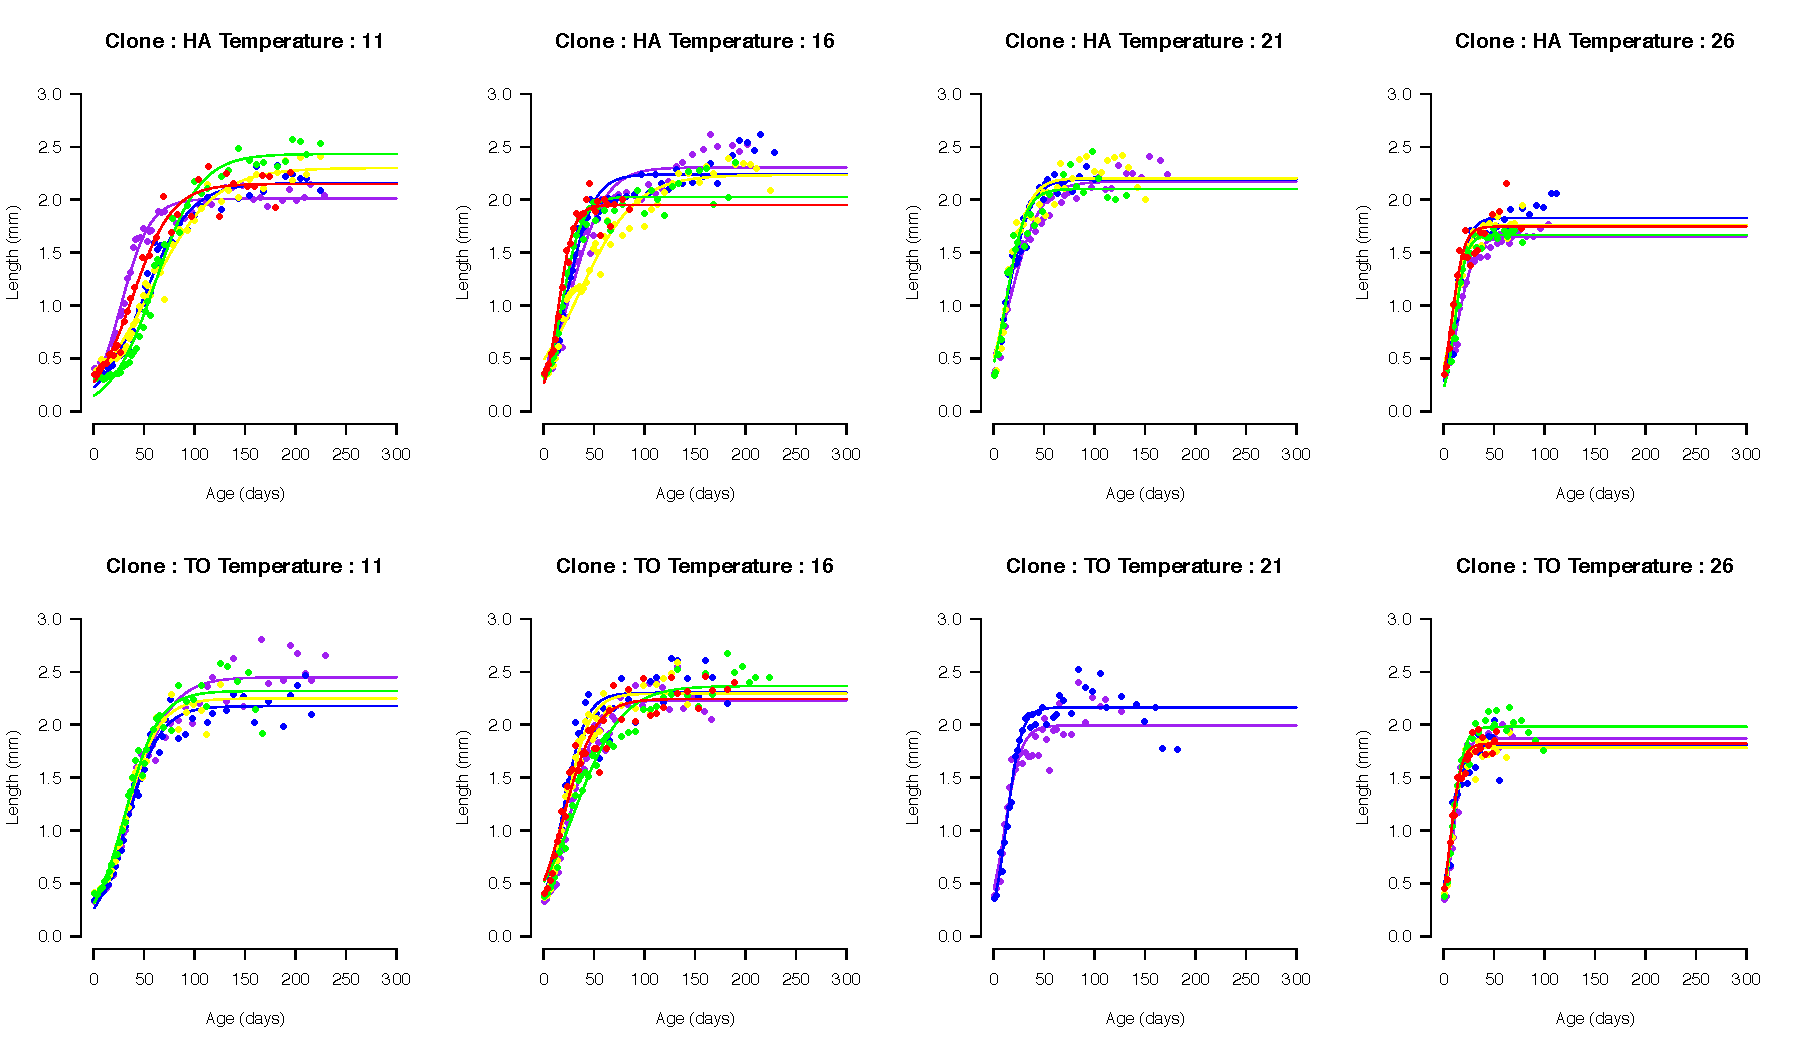
\includegraphics[width=0.95\textwidth]{5_ChapExp3/fig/FigS1}
\caption[\lofimage{5_ChapExp3/fig/FigS1}Individual growth trajectories]{
The 33 individual growth trajectories used to estimate the reaction norms for mean growth rates, size at maturity and adult asymptotic body lengths}
\label{Fig5-S1}
\end{figure}

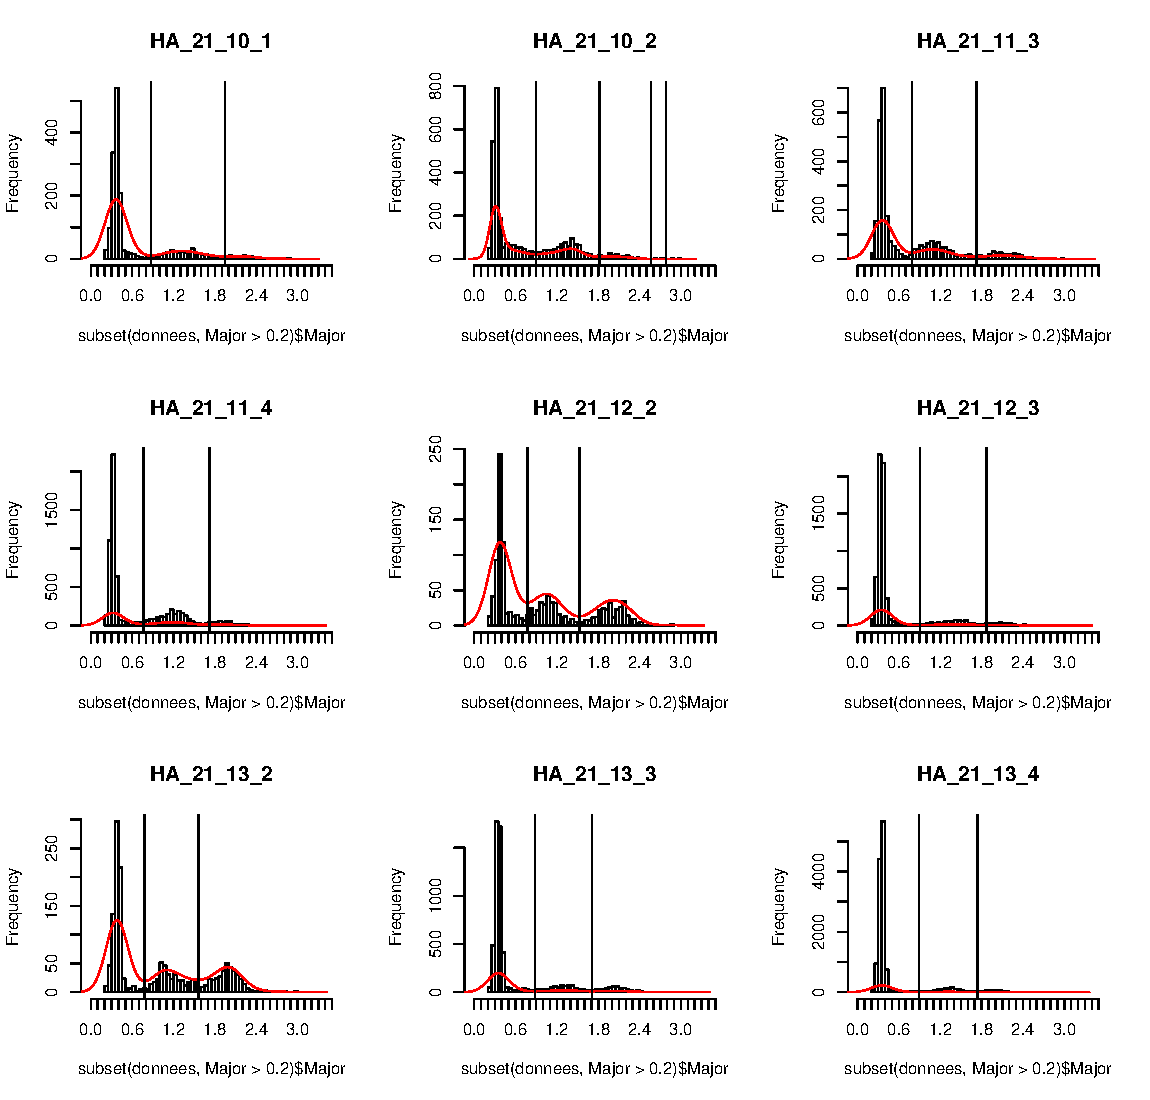
\includepdf[pages=-]{5_ChapExp3/fig/Hist_trimodaux_supp}

 The structure time diagrams of the 46 populations used in our analysis (clones
  TO and HA maintained at 11, 16, 21 and 26$\degres$C). The points underlines the
  measurements of adult body lengths of recently recruited cohorts. The black
  lines show the measures of cohort growth rates in the populations.
  
\includepdf[pages=-]{5_ChapExp3/fig/SupMat3}

